\documentclass[aspectratio=169,11pt]{beamer}

\usetheme{Madrid}
\usecolortheme{default}
\setbeamertemplate{navigation symbols}{}
\setbeamertemplate{footline}[frame number]

\usepackage{amsmath,amssymb}
\usepackage{graphicx}
\usepackage{tikz}
\usetikzlibrary{positioning,calc}
\usetikzlibrary{arrows.meta,decorations.pathmorphing}

\definecolor{RamRed}{RGB}{190,40,45}
\definecolor{RamBlue}{RGB}{30,90,180}
\definecolor{SoftGray}{RGB}{245,245,245}
\definecolor{DarkGray}{RGB}{70,70,70}
\definecolor{MapGreen}{RGB}{48,150,95}
\definecolor{MapGold}{RGB}{235,180,45}

\setbeamercolor{title}{fg=DarkGray}
\setbeamercolor{frametitle}{fg=white,bg=RamBlue}
\setbeamercolor{structure}{fg=RamBlue}

\tikzset{
  v/.style={circle,draw=black,fill=white,inner sep=1.8pt},
  edge/.style={draw=RamBlue,line width=1.25pt},
  topic/.style={draw=black!30,fill=SoftGray,rounded corners=5pt,inner sep=7pt,
    text width=5.8cm,minimum height=1.65cm,align=left},
}


\usepackage{booktabs}
\tikzset{dot/.style={circle,fill=black,inner sep=2pt}, lab/.style={circle,draw=black,fill=white,inner sep=2pt,minimum size=6mm,font=\small},selected/.style={draw=RamRed,line width=2pt}}

\newcommand{\Def}[2]{\begin{block}{#1}#2\end{block}}
\newcommand{\Thm}[2]{\begin{block}{#1}#2\end{block}}
\renewcommand{\Proof}[1]{\begin{block}{Proof}\normalsize #1\end{block}}
\newcommand{\Question}[1]{\begin{block}{Question}#1\end{block}}
\renewcommand{\Example}[1]{\begin{block}{Example}#1\end{block}}
\newcommand{\fall}[2]{#1^{\underline{#2}}}
\newcommand{\rise}[2]{#1^{\overline{#2}}}
\newcommand{\stir}[2]{\left\{\begin{matrix}#1\\#2\end{matrix}\right\}}
\newcommand{\cyc}[2]{\left[\begin{matrix}#1\\#2\end{matrix}\right]}
\newcommand{\eul}[2]{\left\langle\begin{matrix}#1\\#2\end{matrix}\right\rangle}
\newcommand{\coef}[2]{[#1^{#2}]}
\newcommand{\gap}{\par\medskip}

\title{Generating Functions}
\author{Jeremy Quastel}\date{}\begin{document}
\begin{frame}[plain]\begin{center}{\Huge\bfseries Generating Functions}\par\vspace{.25cm}{\Large Section 2.6.1--2.6.3}\par\vspace{.15cm}{\large Harris--Hirst--Mossinghoff, \emph{Combinatorics and Graph Theory}}\par\vspace{.1cm}\resizebox{!}{2.7cm}{\begin{tikzpicture}[x=.65cm]\foreach \i in {1,2,4,5,6,8,9}{\node at (\i,0){$\star$};}\draw[thick](3,-.35)--(3,.35);\draw[thick](7,-.35)--(7,.35);\node at (5,-.8){$2+3+2=7$};\end{tikzpicture}}\par\vspace{.25cm}Jeremy Quastel\end{center}\end{frame}
\begin{frame}[plain]\large \begin{center}{\Huge\bfseries Today\textquotesingle s lecture}\par\vspace{.5cm}\end{center}\begin{columns}[c,onlytextwidth]\begin{column}{.48\textwidth}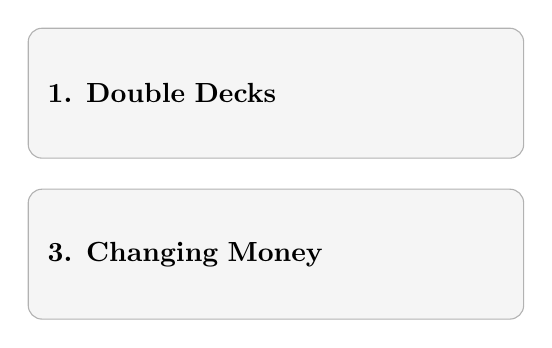
\begin{tikzpicture}\node[topic](a){\textbf{1. Double Decks}};\node[topic,below=.38cm of a]{\textbf{3. Changing Money}};\end{tikzpicture}\end{column}\begin{column}{.48\textwidth}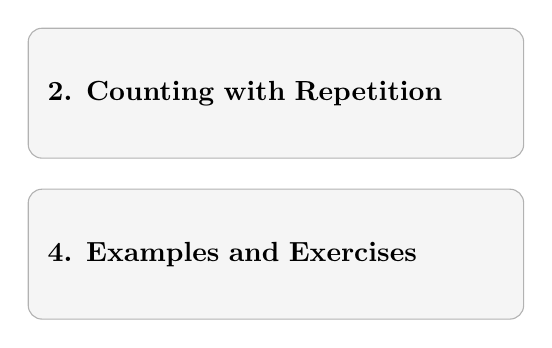
\begin{tikzpicture}\node[topic](a){\textbf{2. Counting with Repetition}};\node[topic,below=.38cm of a]{\textbf{4. Examples and Exercises}};\end{tikzpicture}\end{column}\end{columns}\end{frame}
\begin{frame}{Section 2.6.1: Double decks}
\large
\Question{Suppose two identical copies of each card type are available. How many different hands of a prescribed size can be formed?}
\gap We record card types and multiplicities, not which physical copy was selected.
\gap Ordinary binomial coefficients alone do not account for these repeated types.
\end{frame}
\begin{frame}{A small double deck}
\large
\Example{With two copies each of A, B, and C, the two-card hands are
\[AA,\ AB,\ AC,\ BB,\ BC,\ CC.\]}
\gap Thus there are $6$ hands, not $\binom62=15$. The latter treats the two copies of each type as distinguishable.
\end{frame}
\begin{frame}{A polynomial for one card type}
\large
For each type, choose zero, one, or two copies. Record these choices by
\[1+x+x^2.\]
\gap The exponent records how many cards are selected. The coefficient records how many ways that multiplicity can occur in our model.
\end{frame}
\begin{frame}{Multiplying the choices}
\large
For three card types,
\[(1+x+x^2)^3=1+3x+6x^2+7x^3+6x^4+3x^5+x^6.\]
\gap The coefficient of $x^k$ counts hands of size $k$.
\gap For example, the coefficient $6$ of $x^2$ counts the six hands listed earlier.
\end{frame}
\begin{frame}{Ordinary generating functions}
\large
\Def{Definition}{The ordinary generating function of a sequence $(a_n)_{n\geq0}$ is the formal power series
\[A(x)=\sum_{n\geq0}a_nx^n.\]}
\gap We write $[x^n]A(x)=a_n$ for coefficient extraction.
\end{frame}
\begin{frame}{Formal power series}
\large
\gap Here $x$ is a bookkeeping symbol. We compare coefficients rather than evaluate the series at a real number.
\gap An infinite series is useful when the coefficient of each fixed power can be determined by finitely many relevant choices.
\gap Analytic convergence is a separate question.
\end{frame}
\begin{frame}{Addition and multiplication}
\large
\Thm{Coefficient rules}{If $A(x)=\sum a_nx^n$ and $B(x)=\sum b_nx^n$, then
\[[x^n](A+B)=a_n+b_n,\]
\[[x^n](AB)=\sum_{j=0}^na_jb_{n-j}.\]}
\gap The second formula is the convolution rule.
\end{frame}
\begin{frame}{Why products count combined choices}
\large
\Proof{To form an object of total size $n$ from an A-object and a B-object, choose their sizes $j$ and $n-j$. For that split there are $a_jb_{n-j}$ choices. Sum over all splits.}
\gap Multiplying generating functions combines independent choices and adds their sizes.
\end{frame}
\begin{frame}{The general double-deck answer}
\large
\Thm{Formula}{For $m$ card types with at most two copies of each, the number of hands of size $k$ is
\[[x^k](1+x+x^2)^m.\]}
\gap Each factor corresponds to one distinguishable type.
\end{frame}
\begin{frame}{Counting by the number of pairs}
\large
\Thm{Equivalent formula}{The same number is
\[\sum_{j=0}^{\lfloor k/2\rfloor}\binom mj\binom{m-j}{k-2j},\]
with impossible choices interpreted as zero.}
\Proof{Choose the $j$ types appearing twice, then the $k-2j$ types appearing once. Every hand has a unique number of pairs.}
\end{frame}
\begin{frame}{Five cards from two identical standard decks}
\large
There are $52$ card types. A five-card hand contains zero, one, or two pairs of identical types. Hence its count is
\[\binom{52}5+52\binom{51}3+\binom{52}2\binom{50}1.\]
\gap This equals $[x^5](1+x+x^2)^{52}$.
\end{frame}
\begin{frame}{Symmetry of the coefficients}
\large
\Thm{Observation}{\[[x^k](1+x+x^2)^m=[x^{2m-k}](1+x+x^2)^m.\]}
\Proof{Replace each multiplicity $a_i\in\{0,1,2\}$ by $2-a_i$. A hand of size $k$ becomes a hand of size $2m-k$, and the operation reverses itself.}
\end{frame}
\begin{frame}{Section 2.6.2: Counting with repetition}
\large
\Question{How many multisets of size $n$ can be chosen from $r$ distinguishable types, with unlimited repetition?}
\gap Record the multiplicities $a_1,\ldots,a_r$. The problem is to count
\[a_1+\cdots+a_r=n,\qquad a_i\geq0.\]
\end{frame}
\begin{frame}{Stars and bars}
\large
\begin{center}\begin{tikzpicture}[x=.65cm]\foreach \i in {1,2,4,5,6,8,9}{\node at (\i,0){$\star$};}\draw[thick](3,-.35)--(3,.35);\draw[thick](7,-.35)--(7,.35);\node at (5,-.8){$2+3+2=7$};\end{tikzpicture}\end{center}
\gap Represent $n$ objects by stars and separate the $r$ types by $r-1$ bars. Empty groups are allowed.
\end{frame}
\begin{frame}{The stars-and-bars formula}
\large
\Thm{Theorem}{The number of nonnegative solutions of $a_1+\cdots+a_r=n$ is
\[\binom{n+r-1}{r-1}=\binom{n+r-1}n.\]}
\Proof{A solution is uniquely encoded by $n$ stars and $r-1$ bars. Choose the positions of the bars in a string of length $n+r-1$.}
\end{frame}
\begin{frame}{The geometric series}
\large
\[1+x+x^2+\cdots=\frac1{1-x}.\]
\Proof{Multiplication by $1-x$ cancels every positive-degree term and leaves $1$. This is a formal identity.}
\gap Unlimited copies of one type contribute the factor $(1-x)^{-1}$.
\end{frame}
\begin{frame}{The generating function for repetition}
\large
\Thm{Identity}{\[\frac1{(1-x)^r}=\sum_{n\geq0}\binom{n+r-1}{r-1}x^n.\]}
\Proof{The coefficient in the product of $r$ geometric series counts nonnegative solutions with total $n$. Apply stars and bars.}
\end{frame}
\begin{frame}{Positive multiplicities}
\large
\Thm{Formula}{For $n\geq r$, the number of positive solutions of $a_1+\cdots+a_r=n$ is
\[\binom{n-1}{r-1}.\]}
\Proof{Subtract $1$ from every coordinate, leaving a nonnegative total of $n-r$. Equivalently, use generating function
\[\left(\frac{x}{1-x}\right)^r.\]}
\end{frame}
\begin{frame}{Different lower bounds}
\large
\Question{Count solutions of $a+b+c=12$ with $a\geq2$, $b\geq3$, $c\geq0$.}
\gap Set $a'=a-2$ and $b'=b-3$. Then $a'+b'+c=7$, so the answer is
\[\binom92=36.\]
\gap The generating function is $x^5/(1-x)^3$.
\end{frame}
\begin{frame}{Upper bounds}
\large
\Thm{Generating function}{The number of solutions of $a_1+\cdots+a_r=n$ with $0\leq a_i\leq b_i$ is
\[[x^n]\prod_{i=1}^r(1+x+\cdots+x^{b_i}).\]}
\gap Each factor lists exactly the allowed values of one coordinate.
\end{frame}
\begin{frame}{Recovering inclusion and exclusion}
\large
When every upper bound is $b$,
\[(1+x+\cdots+x^b)^r=\frac{(1-x^{b+1})^r}{(1-x)^r}.\]
Expand the numerator by the binomial theorem and the denominator by stars and bars. The coefficient of $x^n$ is
\[\sum_{j=0}^{\min(r,\lfloor n/(b+1)\rfloor)}(-1)^j\binom rj
\binom{n-j(b+1)+r-1}{r-1}.\]
\end{frame}
\begin{frame}{Parity restrictions}
\large
\Example{Count solutions of $a+b+c=8$ with $a$ even and $b,c\geq0$.}
\gap Use
\[\frac1{(1-x^2)(1-x)^2}.\]
\gap Summing over $a=0,2,4,6,8$ gives $9+7+5+3+1=25$.
\end{frame}
\begin{frame}{Section 2.6.3: Changing money}
\large
\Question{How many ways can a sum be formed using coins of specified denominations?}
\gap Coins of the same denomination are indistinguishable. Order does not matter.
\gap A denomination $d$ contributes
\[1+x^d+x^{2d}+\cdots=\frac1{1-x^d}.\]
\end{frame}
\begin{frame}{The coin generating function}
\large
\Thm{Formula}{For unlimited coins of denominations $d_1,\ldots,d_r$, the number of ways to form amount $n$ is
\[[x^n]\prod_{i=1}^r\frac1{1-x^{d_i}}.\]}
\gap The exponent records value, rather than the number of coins.
\end{frame}
\begin{frame}{Coins of values $1$, $2$, and $5$}
\large
\Question{How many ways can these coins make $10$ units?}
\gap Solve $a+2b+5c=10$ in nonnegative integers.
\begin{center}\begin{tabular}{c|c|c}
$c$ & Remaining value & Choices for $b$\\\hline
0&10&6\\1&5&3\\2&0&1
\end{tabular}\end{center}
\gap Total: $6+3+1=10$.
\end{frame}
\begin{frame}{A coefficient version of the calculation}
\large
\[[x^{10}]\frac1{(1-x)(1-x^2)(1-x^5)}=10.\]
\gap With only values $1$ and $2$, amount $m$ can be formed in $\lfloor m/2\rfloor+1$ ways.
\gap Sum this count for remaining amounts $10,5,0$ after choosing the number of $5$-coins.
\end{frame}
\begin{frame}{Several denominations}
\large
For denominations $1,5,10,25,50,100$, the generating function is
\[\frac1{(1-x)(1-x^5)(1-x^{10})(1-x^{25})(1-x^{50})(1-x^{100})}.\]
\gap Only terms up to the desired amount are needed when computing a coefficient.
\end{frame}
\begin{frame}{A recurrence for changing money}
\large
\Def{Notation}{Let $f_j(n)$ count ways to form $n$ using the first $j$ denominations. Set $f_j(n)=0$ for $n<0$.}
\Thm{Recurrence}{\[f_j(n)=f_{j-1}(n)+f_j(n-d_j).\]}
\gap The two terms count choices using no $d_j$-coin and choices using at least one $d_j$-coin.
\end{frame}
\begin{frame}{Initial conditions}
\large
\[f_0(0)=1,\qquad f_0(n)=0\quad(n>0).\]
\gap The empty collection is the unique way to form zero. These initial conditions and the recurrence determine all counts.
\gap Removing one $d_j$-coin from a collection in the second case explains why that term still allows all $j$ denominations.
\end{frame}
\begin{frame}{Does order matter?}
\large
\Question{How many ways can $4$ be written using parts $1$ and $2$?}
\gap Unordered: $1+1+1+1$, $2+1+1$, $2+2$, giving $3$.
\gap Ordered: $1111$, $112$, $121$, $211$, $22$, giving $5$.
\gap The product $1/((1-x)(1-x^2))$ counts the unordered version.
\end{frame}
\begin{frame}{Practice}
\large
\Question{Find the number of solutions of $a+b+c=10$ with $a\geq1$, $0\leq b\leq3$, and $c$ even.}
\gap Write a generating function, then count directly by the value of $c$.
\end{frame}
\begin{frame}{Practice: solution}
\large
\normalsize
The generating function is
\[\frac{x(1+x+x^2+x^3)}{(1-x)(1-x^2)}.\]
For $c=0,2,4,6$, each of $b=0,1,2,3$ gives a positive $a$. For $c=8$, only $b=0,1$ work. For $c=10$, none work.
\[4+4+4+4+2=18.\]
\end{frame}
\begin{frame}{Summary}
\large
\begin{itemize}
\item A generating function records counts as coefficients.
\item Products combine independent choices and add sizes.
\item Repetition and bounds are encoded by geometric-series factors.
\item Coin problems use exponents for total value and distinguish order from multiplicity.
\end{itemize}
\end{frame}
\begin{frame}{Next time: Fibonacci Numbers and Recurrences}\begin{center}{\Huge Fibonacci Numbers and Recurrences}\end{center}\end{frame}
\end{document}